\chapter{Stand van zaken}
\label{ch:stand-van-zaken}

% Tip: Begin elk hoofdstuk met een paragraaf inleiding die beschrijft hoe
% dit hoofdstuk past binnen het geheel van de bachelorproef. Geef in het
% bijzonder aan wat de link is met het vorige en volgende hoofdstuk.

% Pas na deze inleidende paragraaf komt de eerste sectiehoofding.

Dit hoofdstuk bevat een literatuurstudie omtrent data warehousing. Na het lezen van dit hoofdstuk zullen begrippen zoals dimensioneel modelleren, data vault 2.0 en data warehousing jou niet meer onbekend zijn en waarom er nood is aan data warehousing. Ook zullen beide modelleertechnieken dieper bekeken worden.

%\textcite{Knuth1998}
\section{Inleiding data warehousing}

\epigraph{Torture the data, and it will confess to anything. }{\textit{Ronald Coase \\ Winnaar Nobelprijs in Economie (1991)}}

Veel moderne, digitale bedrijven genereren tegenwoordig enorme volumes data. Deze data kan afkomstig zijn uit verschillende bronnen: CRM-systeem, flat-files (vb. rekenbladen), Twitter-feeds, ... Bestuursleden gebruiken data om beslissingen te nemen die de onderneming toelaat om te (blijven) groeien of om bepaalde problemen op te sporen. Stel dat een onderneming meer kosten maakt dan opbrengsten. Op basis van alle gegevens die het bedrijf bezit, kan hieruit dan een analyse gemaakt worden. Zijn er overbodige kosten? Worden onze producten/diensten aan een te lage prijs verkocht? Dit zijn maar enkele vragen die kunnen opgelost worden wanneer het bestuur de correcte rapporteringen ontvangt. 

\subsection{Soorten data}
Er kan een onderscheid gemaakt worden tussen verschillende soorten data. Voornamelijk kunnen we informatie opdelen in 2 categorieën: gestructureerde en ongestructureerde data. Volgens een artikel van ~\textcite{Langseth2005}, bestaat 95\% van de globale informatie uit ongestructureerde data. 

\subsubsection{Gestructureerde data}
Data afkomstig uit een relationele databank (RDBMS) is meestal gestructureerd. Deze data is meestal ingedeeld in categorieën, denk bijvoorbeeld maar aan postcode, naam, klantennummer, ... Hieruit volgt dat deze data heel gemakkelijk te doorzoeken is. 

\subsubsection{Ongestructureerde data}
Deze informatie kan niet gemakkelijk worden opgeslagen in databanken. Denk maar aan rekenbladen, emails, tweets, muziek, ... Data afkomstig uit IoT-apparaten zijn meestal ook ongestructureerd. Deze data bevat vaak ook heel nuttige informatie die organisaties graag willen benuttigen. Denk bijvoorbeeld maar aan tweets: hoe gelukkig zijn klanten over een bepaald product? Hoeveel mails worden er maandelijks ontvangen met klachten?

\subsection{Wat is een data warehouse?}
De definitie van een data warehouse luidt als volgt: \textit{"een subject-georiënteerde, geïntegreerde, tijd-variante, niet-vluchtige collectie van gegevens dat in eerste instantie gebruikt wordt bij organisaties om beslissingen te nemen"} ~\autocite{Panos2000}.

\paragraph{Subject-georiënteerd}
Dit begrip slaat op het feit dat een data warehouse met de reden gebouwd is om data te analyseren, niet om transacties op toe te passen. Dit wordt uitgebreid besproken in subsectie \ref{sec:oltp-vs-olap}.


\paragraph{Geïntegreerd}
Dit betekent dat de data warehouse een "centrale" databank is die gegevens bevat vanuit verschillende bronsystemen (bijvoorbeeld gegevens uit het klantenbestand en gegevens uit het verkoopsysteem). Deze data kan effectief ingeladen worden, maar ook opgeslagen worden in virtuele tabellen.

\paragraph{Tijd-variant}
Alle data van het verleden, moet terug te vinden zijn in de data warehouse. Dit betekent dat data uit het verleden (bijvoorbeeld een vorig adres van een klant) moet beschikbaar zijn, ook al is deze in het transactioneel systeem aangepast.

\paragraph{Niet-vluchtig}
De data die in het systeem zit, moet onveranderlijk zijn, ook al zijn deze fout. Om de foutieve data toch aan te passen, zal er een nieuwe rij moeten toegevoegd worden die de juiste data bevat, die een hogere versie bevat dan de vorige rij. 

\paragraph{Conclusie}
We kunnen dus uit de definitie van een data warehouse afleiden dat het een grote databron is die alle (gestructureerde en ongestructureerde (indien mogelijk)) gegevens bevat die een organisatie bezit vanaf het moment waarbij de data warehouse geïmplementeerd is tot het heden. Op deze databron worden dan analyses gemaakt.

\subsection{Waarom is er nood aan een data warehouse?}
Een organisatie heeft tegenwoordig heel wat data ter beschikking. Vaak is deze data gefragmenteerd over verschillende systemen. Wanneer men een analyse wil opmaken op basis van de verspreide data, zal dat niet evident zijn. 

Om deze reden wordt een data warehouse ontworpen. Hierin worden gegevens, verspreidt over meerdere bronnen, in één bron verzameld. Zo kunnen rapporteringen makkelijk en flexibel opgebouwd worden. 

Een andere reden voor het opbouwen van een data warehouse is dat je de historiek van alle data kan bijhouden. Wanneer er bijvoorbeeld gegevens aangepast zijn in het transactionele systeem, dan zijn de oude gegevens vaak moeilijk te achterhalen (omdat deze dat vaak overschreven wordt). Door verschillende versies bij te houden van entiteiten, kan je oudere data makkelijk opzoeken.

Wanneer men rapporteringen wil opvragen aan het transactionele systeem, vergt dit ook extra belasting van de server. Dit komt doordat het datamodel die opgebouwd werd niet geoptimaliseerd is om zware SELECT-queries af te handelen. Dit zou niet alleen de server meer belasten, bovendien zal dit ook zorgen voor een tragere rapportering. 


\subsection{Wat is het doel van een data warehouse?}
Het belangrijkste doel dat een data warehouse heeft is om een \textbf{correcte} rapportering op te leveren. Beslissingen in organisaties worden genomen op basis van rapporten.

\paragraph{Data kwaliteit}
Zoals eerder aangekaart, is het belangrijk dat rapporten de juiste gegevens bevat. Hieruit volgt dat data kwaliteit een heel belangrijk aspect is. Vaak zijn er verschillende oorzaken waarom de data kwaliteit niet voldoet:

\begin{itemize}
	\item Inconsistente data tussen verschillende systemen
	\item Incorrecte gegevens
	\item Onvoldoende validatie bij het invoeren van gegevens
	\item Onjuiste gegevensbewerkingen
	\item \ldots
\end{itemize}  
~\autocite{Helfert2002}

Gegevens die in een data warehouse geladen worden, ondergaan een proces (zie paragraaf \ref{sec:etl}). In dit proces wordt de data gemanipuleerd zodat de data kwaliteit verhoogd wordt.

\paragraph{Performantie}
We kunnen een onderscheid maken tussen 3 verschillende soorten beslissingen: operationele (dagelijks), tactische (jaarlijks) en strategische (lange termijn) beslissingen. Wanneer we operationele rapporten nodig hebben, verwachten we dan ook dat deze onmiddelijk kunnen opgeleverd worden. Het datamodel van een data warehouse wordt geoptimaliseerd voor het ophalen van data in plaats van het te kunnen stockeren. De data wordt 's nachts ingeladen zodat werknemers geen performantieproblemen hieromtrend ondervinden. 

\subparagraph{De toekomst}
Door de komst van in-memory databanken merken we op dat een deel van de (operationele) rapportering opnieuw verhuist naar de transactionele databanken. Dit heeft enerzijds te maken met de snelheid van de databanken en anderzijds met het feit dat queries om operationele rapporten op te vragen gebruikelijk niet zo belastend zijn. Zo kan er gewerkt worden met \textbf{live data} (doordat deze niet 's nachts moet ingeladen worden in de data warehouse). De voorwaarde hiervoor is dat alle benodigde data beschikbaar is binnen dat geïntegreerd systeem. Een voorbeeld van een in-memory databank is HANA, een technologie ontwikkelt door SAP.

\paragraph{Automatisering}
Doordat alle rapporteringsnoden geautomatiseerd kunnen worden, heeft dit natuurlijk als voordeel dat personeelsleden deze niet meer manueel hoeven te maken/berekenen. Zo kunnen ze hun tijd spenderen aan andere prioriteiten. Deze data kan dan worden voorgesteld in een overzichtelijke omgeving (zie sectie \ref{sec:omgeving}).

\subsection{Wat is OLTP en wat zijn de verschillen met OLAP?}
\label{sec:oltp-vs-olap}
On-line transactional processing (OLTP) systemen zijn voornamelijk klantgericht. Het datamodel is opgebouwd rond het efficiënt verwerken van transacties. On-line analytical processing (OLAP) systemen zijn martkgericht. De data in een OLAP-systemen worden gebruikt om analyses op uit te voeren ~\autocite{Satyanarayana2010}.


\paragraph{Inhoudelijk}
Bij OLAP systemen worden meta data opgeslagen bij de entiteiten. Voorbeelden hiervan zijn: tijdstip van inladen, van welke bron de data komt, ... Het grote voordeel hierbij is dat wanneer een fout gebeurt, er gemakkelijker kan achterhaalt worden waar het fout liep. Ook wordt de historische data ook bewaard, in tegenstelling tot OLTP. Bij OLTP wordt de te wijzigen data overschreven. Het gevolg hiervan is dat de volume data bij OLAP doorgaans groter zal zijn.

\paragraph{Toegankelijkheid}
Wanneer men data wil verkrijgen/wijzigen in een OLTP systeem, moet er rekening gehouden met een aantal aspecten. Een transactie in een OLTP omgeving moet voldoen aan enkele eisen:
\begin{itemize}
	\item \textbf{Atomic:} Wanneer een transactie afgebroken is, mag er niets gewijzigd zijn in de databank.
	\item \textbf{Consistent:} Als een deel van de transactie faalt, zullen alle doorgevoerde wijzigingen in die transactie ongedaan gemaakt worden en zal de databank terugkeren naar een consistente staat.
	\item \textbf{Isolated:} Transacties worden geïsoleerd, transacties mogen in geen enkel geval elkaar beïnvloeden.
	\item \textbf{Durable:} Wanneer een transactie is doorgevoerd, kan deze niet meer ongedaan gemaakt worden.
\end{itemize}  

Bij een OLAP-systeem worden geen transacties doorgevoerd, enkel leesopdrachten. Dat vermindert de complexiteit en verhoogt de snelheid van de queries ~\autocite{Satyanarayana2010}. 

\subsection{Wat zijn de benodigdheden voor een data warehouse?}
Voor er kan begonnen worden met het opbouwen van een data warehouse, zijn er enkele benodigdheden. Zo zal er een keuze moeten gemaakt worden voor een bepaalde methodologie en een architectuur. Ook zal er fysieke opslagplaats nodig zijn. Hiervoor kan gebruik gemaakt worden van Cloud oplossingen of een on-premise server. Maar in dit hoofdstuk bespreken we welke software-aspecten er nodig zijn bij het opbouwen van de data warehouse.

\subsubsection{RDBMS}
Voor het opmaken en beheren van de data warehouse zal er een RDBMS moeten uitgekozen worden. Hiervoor zijn heel wat mogelijkheden beschikbaar op de markt. Bijvoorbeeld: 

\begin{itemize}
	\item Oracle DB
	\item Microsoft SQL Server
	\item IBM DB2
	\item Microsoft Office Access
	\item \ldots
\end{itemize} 

Klassieke databanken slaan hun gegevens op op harde schijven en/of SSD's. Maar sinds kort zien we de komst van een nieuwe technologie, genaamd een in-memory databank. Hierbij worden de gegevens initieël opgeslagen in het RAM-geheugen. Dit zorgt voor een veel snellere lees- en schrijftijd. Het nadeel van deze nieuwe technologie is het prijskaartje.

\subsubsection{Data integratie software}
\label{sec:etl}
Het data inladen is een proces die een verantwoordelijkheid is voor de data integratie software, al is dat niet zijn enige verantwoordelijkheid. Hij is verantwoordelijk voor het gehele ETL-proces:

\begin{itemize}
	\item Extraction: Ophalen van de data vanuit de bron
	\item Load: Transformaties en manipulaties uitvoeren op die data
	\item Transformation: De data wegschrijven naar de nieuwe bron
\end{itemize} 

\section{Dimensioneel modelleren via Kimball}
Wie een consultant Business Intelligence is, heeft ongetwijfeld al gehoord van dimensioneel modelleren. Over de jaren heen is het als het ware een standaard geworden wanneer men een data warehouse wilt ontwerpen. Dimensioneel modelleren heeft als voordeel dat het model niet complex is, dus gemakkelijk te begrijpen, zelf voor niet IT-opgeleide personen. Ook is er vaak een snel resultaat beschikbaar. In deze sectie zal het dimensioneel modelleren aan de hand van Kimball dieper bekeken worden. 


\subsection{Architectuur}
Bij het dimensioneel modelleren wordt het proces opgedeeld in 2 soorten lagen:de data warehouselaag en de data marts. Op basis van de data warheouselaag worden de data marts opgebouwd. Rapporteringsomgevingen connecteren met de data marts om hun data op te halen.

\subsubsection{Data warehouselaag}
In deze laag wordt het ETL-proces toegepast. Eerst en vooral wordt de data vanuit (een) bron(nen) in de warehouse geladen. Daarna wordt de data bewerkt en gemanipuleerd. Bijvoorbeeld records met bepaalde lege records weglaten. De data kwaliteit (zoals eerder aangekaart) is zeer belangrijk in een data warehouse. Het doel is om de toegekomen data consistent te maken en ervoor te zorgen dat de integriteit bewaarborgd blijft ~\autocite{Kimball2013}

\subsubsection{Data marts}
In deze laag worden OLAP-cubes of relationele ster schema's gemaakt op basis van de data warehouselaag. Deze laag kan eigenlijk als de presentatielaag beschouwd worden. Deze laag moet gedetailleerde data bevatten. Een data mart moet gebaseerd zijn rond een business unit ~\autocite{Kimball2013}.

\subsection{Componenten}
Een sterschema of OLAP-cube bestaat uit dimensies en facts. Wat deze precies zijn, wordt hieronder uitgelegd. 

\subsubsection{Dimention tabel}
Voor elke dimensie wordt een primaire sleutel aangemaakt (of afkomstig uit het systeem als business sleutel). Deze sleutel wordt gebruikt in een fact table als vreemde sleutel, zodat er een relatie kan worden gelegd tussen beide entiteiten.

Naast de primaire sleutel wordt in deze tabel ook de beschrijvende data bewaart voor een bepaalde rij. Deze data kan gebruikt worden om in de rapporteringsomgeving de verschillende assen te kiezen. Een typische dimensie is bijvoorbeeld 'naam' of 'Woonplaats'.

\subsubsection{Fact tabel}
In een fact table worden alle meetbare cijfers bijgehouden. Meetbare cijfers betekent dat bewerkingen moeten kunnen mogelijk zijn op die data. Een bankrekeningnummer is een getal, maar hier kunnen geen bewerkingen met uitgevoerd worden (bijvoorbeeld gemiddelde bankrekeningnummer geven). Invoice amount is wel een goed voorbeeld. Hierop kunnen enkele bewerkingen worden uitgevoerd, bijvoorbeeld: gemiddelde, minimum, maximum, totaal, .... Deze gegevens worden in vaktermen als \textbf{measures} aangeduidt. 

De fact table bevat niet alleen measures, maar ook de vreemde sleutels van de dimensies waarmee het verbonden is. Zo kan je bruikbare informatie toevoegen aan je measure in de rapporteringsomgeving.

\subsubsection{Ster schema}
In een ster schema worden dimensies en fact tabellen verbonden door enerzijds de primaire sleutels in de dimensies, en anderzijds bij de vreemde sleutels in de fact tabel. Wanneer meerdere tabellen verbonden worden met elkaar zien we een centraal punt in het model, dat de fact tabel is (zie figuur \ref{fig:ster}). 

\begin{figure}[h]
	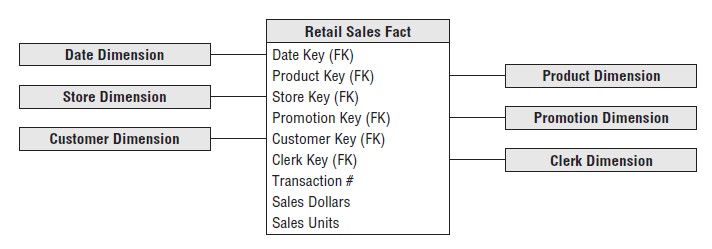
\includegraphics[scale=0.8]{../images/ster.PNG}
	\caption{Ster sschema voorgesteld door \textcite{Kimball2013}.}
	\label{fig:ster}
\end{figure}

\subsubsection{Verschil tussen een sterschema en een OLAP-cube}
Het verschil tussen beide zit niet in het ontwerp, maar puur in het 'fysieke' gedeelte.
OLAP cubes zijn geoptimaliseerd voor een drill down of een frill up te doen in de gegevensset.
Drill down betekent dat de gegevens op een dieper detailniveau zullen bekeken worden, bijvoorbeeld vertrekkend uit een productcategorie niveau, ga je naar een productniveau. OLAP cubes zorgen ervoor dat er meer anlytische functies beschikbaar zijn in vergelijking met SQL. Maar als nadeel heeft de OLAP cubes dat het niet zo performant is als een ster schema  (zie figuur \ref{fig:stervsolap}).  \autocite{Kimball2013}. 

\begin{figure}[h]
	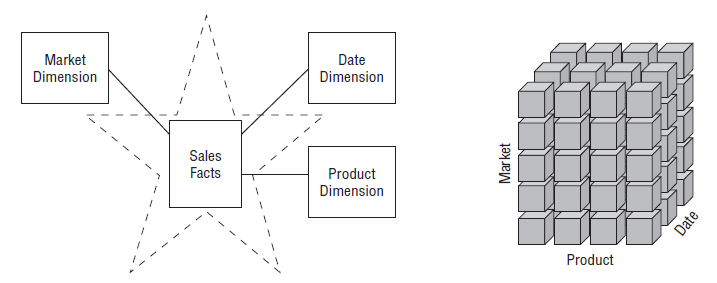
\includegraphics[scale=0.8]{../images/starvsolap.PNG}
	\caption{Sterschema (links) en OLAP cube (rechts) voorgesteld door \textcite{Kimball2013}.}
	\label{fig:stervsolap}
\end{figure}

\section{Modelleren via Data Vault 2.0}
Data Vault 2.0 is een modelleertechniek die ontworpen is door Daniel Linstedt. Het model zorgt ervoor dat dimensies gemakkelijk uitgebreidt kunnen worden en dat databronnen toevoegen vlot moet gaan. Linstedt is van mening dat business requirements vaak veranderen, dus moet het model waarin de data warehouse ontworpen is ook flexibel zijn. 
~\autocite{Linstedt2016}
\subsection{Architectuur}
Data vault maakt gebruik van een 3-lagen model. Dit heeft als voordeel dat processen duidelijk kunnen onderscheiden worden per laag en blijft alles overzichtelijk. Deze architectuur ondersteunt om data op halen via een batch, maar ook om live data op te halen. NoSQL kan ook gebruikt worden om de data warehouse te ontwerpen. Wanneer de data live opgehaald wordt, valt de staging area weg en wordt de data onmiddelijk in de raw data vault geladen.  ~\autocite{Linstedt2016}


\begin{figure}[h]
	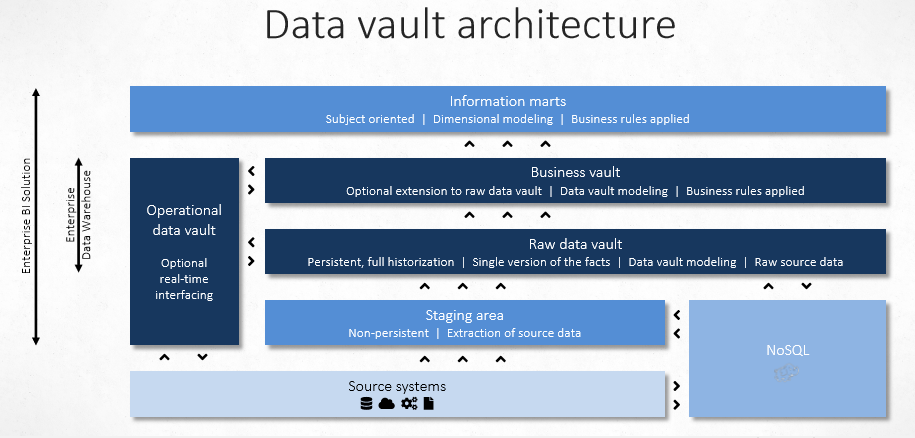
\includegraphics[scale=0.63]{../images/DVArchitectuur.png}
	\caption{Data Vault architectuur voorgesteld door \textcite{Stroobants2018}.}
	\label{fig:dvarch}
\end{figure}

\subsubsection{Staging area}
In deze laag wordt alle data ingeladen (of een virtuele tabel gebruikt) van een bepaalde bron via een batch. Hier wordt alle data onbewerkt ingeladen. Deze data bevat dan ook nog geen historische data. De tabel worden dus gedupliceerd van de bron(nen). Deze laag is niet persistent.

\subsubsection{Raw data vault}
De data wordt overgeladen van de staging area naar de raw data vault via data integratie software. Deze laag is persistent, logisch ook wanneer we verschillende versies en de historiek behouden van onze entiteiten. Vanaf deze laag beginnen we te modelleren in Data Vault. De data wordt in deze laag gemanipuleerd (ofwel getransformeerd (ETL)). Ook wordt er metadata toegevoegd aan de records zodat er audits kunnen plaatsvinden. 

\subsubsection{Business vault}
Dit is een optionele laag. Deze laag wordt enkel en alleen toegevoegd wanneer er 'Business regels' moet toegepast worden in het model. De business vault wordt in princiepe niet opgeslagen in een aparte laag, maar vaak wordt deze opgeslagen als een uitbreiding van de raw data vault. Een voorbeeld van een 'Business rule' is dat je bijvoorbeeld geen producten wil promoten wanneer er maar minder dan 10 in voorraad zijn.

\subsubsection{Information marts}
Vertrekkend uit de business vault (of raw data vault wanneer deze niet aanwezig is) zullen er information marts moeten aangemaakt worden, ook wel bekend als data marts . ~\textcite{Linstedt2016} spreek liever over 'information' mart omdat het doel van een enterprise data warehouse duidelijk is: informatie aanbieden. 
De information marts bestaan uit sterschema's. Hierop connecteren de eindgebruikers om hun informatie te verschaffen. 

\subsection{Componenten}
Een data vault model bestaat uit 3 soorten componenten: hubs, links en sattelieten. Elk component heeft zijn functie en zijn doel.

\subsubsection{Hubs}
~\textcite{Linstedt2016} beschrijft hubs als pilaren voor het Data Vault model. Een hub bestaat altijd uit minmaal 4 attributen:

\begin{itemize}
	\item \textbf{Hashkey (PK):} Als primaire sleutel van de entiteit wordt een gehashte identifier van de entiteit gebruikt.
	\item \textbf{LoadDate:} Datum/tijdstip wanneer de record is ingeladen
	\item \textbf{Record source:} Van welke databron is de record afkomstig?
	\item \textbf{Business key(s):} De business key(s) van de bijhorende entiteit
\end{itemize} 

 De business key is een unieke sleutel, die vaak een betekenis heeft naar de business. Voorbeelden zijn: ISBN-nummers, Klantnummer, Chassisnummer, ...
 
 Hubs zijn vooral heel handig wanneer er meerdere databronnen zullen zijn, zo kan je meerdere bronnen aan een hub hangen. In een hubs zit nooit andere data buiten een hash key, metadata en business keys.

\subsubsection{Links}
Wanneer we 2 hub-entiteiten willen verbinden, zullen we ze niet rechtstreeks met elkaar verbinden. Twee hub-entiteiten worden namelijk verbonden door middel van een link. Andere verantwoordelijkheden voor een link zijn hierarchieën, redefinities of business termen. De bedoeling is om een zo laag mogelijke granulariteit te creeëren. Links zorgen ervoor dat het data vault model heel flexibel wordt en makkelijk uitbreidbaar is. 

\begin{figure}[h]
	\centering
	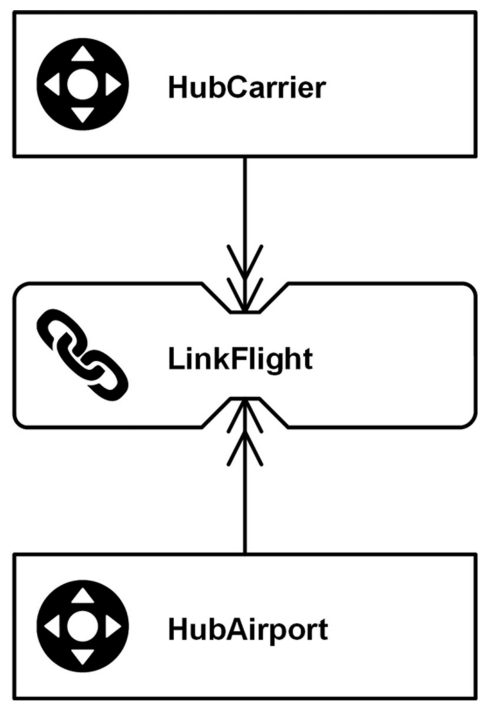
\includegraphics[scale=0.3]{../images/link.png}
	\caption{Link entiteit die 2 hub entiteiten met elkaar verbindt. \autocite{Linstedt2016}.}
	\label{fig:link}
\end{figure}

Ook bij links moeten er een aantal attributen aanwezig zijn:

\begin{itemize}
	\item \textbf{Hashkey (PK):} Als primaire sleutel van de entiteit worden alle business keys gehasht naar 1 sleutel.
	\item \textbf{LoadDate:} Datum/tijdstip wanneer de record is ingeladen
	\item \textbf{Record source:} Van welke databron is de record afkomstig?
	\item \textbf{Business key(s):} Alle business key(s) van de 2 gelinkte hub-entiteiten
\end{itemize} 

\subsubsection{Sattelieten}
In een satteliet worden alle gegevens gestockeerd dat een business object, relatie of transactie beschrijft. In de entiteit zelf is het belangrijk dat de historiek wordt bijgehouden. \autocite{Linstedt2016}

Bij een satteliet vinden we minstens volgende attributen terug:

\begin{itemize}
	\item \textbf{Parent Hashkey (PK):} Als primaire sleutel van de entiteit worden alle business keys gehasht naar 1 sleutel.
	\item \textbf{LoadDate:} Datum/tijdstip wanneer de record is ingeladen
	\item \textbf{Record source:} Van welke databron is de record afkomstig?
	\item \textbf{End load date:} Hierin wordt het moment geladen wanneer de entiteit niet meer gebruikt wordt (belangrijk voor het bewaren van de historiek).
\end{itemize} 

Een satteliet hoort bij een hub of een link. Een hub en een satteliet vormen een bepaald business object. 

\subsubsection{Data Vault schema}
Wanneer we zowel hubs, links als sattelieten samengieten in één schema, bekomen we een data vault. Wel zijn er nog enkele belangrijke opmerkingen:

\begin{itemize}
	\item Hubs mogen nooit rechtstreeks verbonden met elkaar, dit moet altijd gebeuren via een link (anders verliest het model zijn flexibiliteit).
	\item Sattelieten kunnen zowel met hubs als links verbonden worden.
	\item Hubs/links kunnen meerdere sattelieten hebben: deze staan meestal voor verschillende databronnen.
	\item Een satteliet kan maar verbonden worden met 1 hub of link. 
\end{itemize} 

\begin{figure}[h]
	\centering
	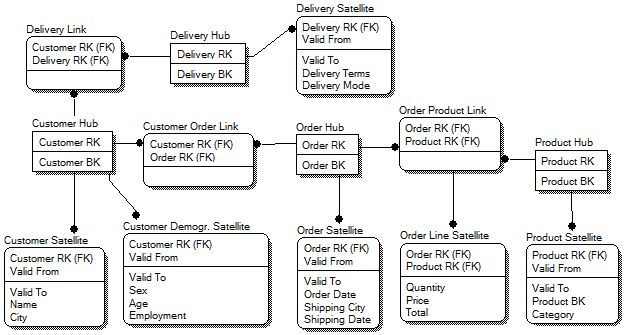
\includegraphics[scale=0.7]{../images/dvmodel.png}
	\caption{Een voorbeeld van een data vault model (Bukhantsov.org)}
	\label{fig:dvmod}
\end{figure}

Dit model heeft veel flexibiliteit te bieden. Enerzijds kan er gemakkelijk nieuwe hubs toevoegen door een nieuwe link te leggen. Ook kan er heel gemakkelijk een nieuwe gegevensbron toevoegen, dit wordt gedaan door een nieuwe satteliet toe te voegen aan een bestaande hub. 

\section{Rapporteringsomgevingen}
\label{sec:omgeving}
Wanneer alle data in de data warehouse ingeladen en getransformeerd is, moet het mogelijk zijn om visuele en interactieve rapporten op te stellen. Op basis van deze rapporten, kan het beleid beslissingen gaan nemen. Ook kunnen dashboards opgesteld worden voor werknemers die geen beleid voeren. De bedoeling in deze sectie is om een schets te geven over welke rapporteringsomgevingen op de markt beschikbaar zijn. 

\subsection{SAP Analytics Cloud}
Bij SAP Analytics Cloud kan er gebruik gemaakt worden van realtime analytics. Hiervoor is live data nodig en deze wordt opgehaald in het transactionele systeem. Indien gewenst, kan er toch nog steeds gewerkt worden met een batch die 's nachts geladen wordt. 

Analytics cloud biedt heel veel mogelijkheden om interactieve dashboards te ontwerpen. Waar SAP Analytics Cloud zich onderscheidt met de andere spelers, is dat er in deze omgeving planning kan worden toegepast. Er kunnen budgetten opgesteld worden voor de komende jaren (bijvoorbeeld IT-kosten), en deze kunnen dan vergeleken worden met de actuele kosten op dat momenten. Wanneer een bedrijf deze planning-feature wil implementeren, moeten ze hiervoor een pak meer geld op tafel leggen. 

\begin{figure}[h]
	\centering
	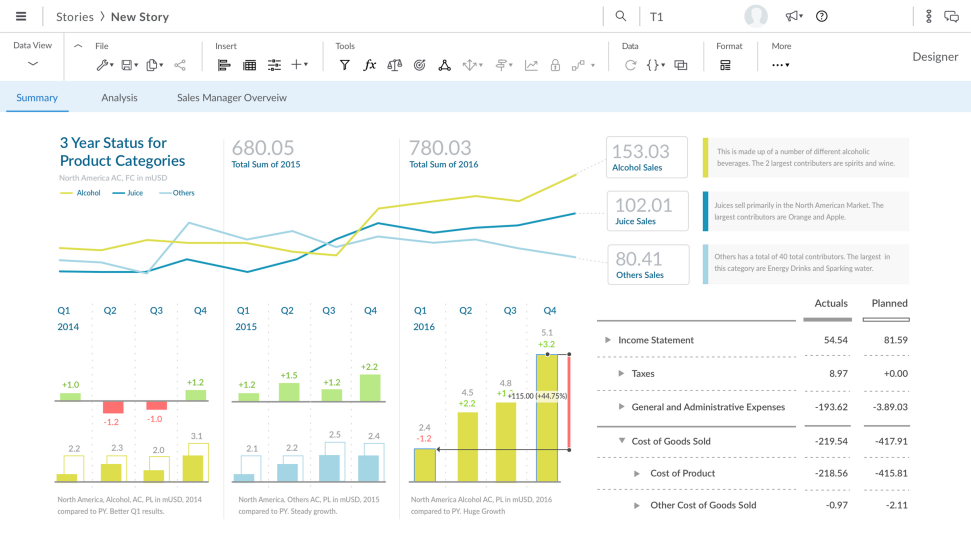
\includegraphics[scale=0.45]{../images/sac.png}
	\caption{Een voorbeeld van een dashboard gemaakt met SAP Analytics Cloud (sap.com)}
	\label{fig:sac}
\end{figure}

\subsection{Power BI}
Power BI is het programma bij uitstek die gebruikt wordt bij datavisualisatie van ontwikkelaar Microsoft. PowerBI is een uitstekende keuze wanneer bedrijven Office 365 en microsoft Dynamics geïmplementeerd hebben in hun infrastructuur.

In tegenstelling tot SAP Analytics cloud kan je Power BI wel on-premise installeren. Maar indien gewenst, kan er steeds gebruikt gemaakt worden van een cloud-omgeving.

\begin{figure}[h]
	\centering
	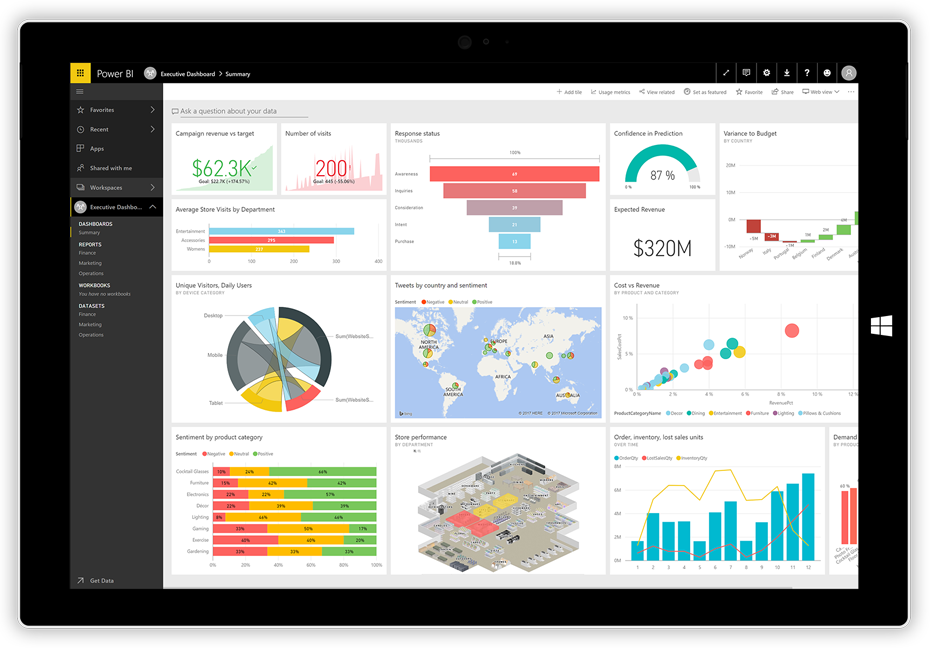
\includegraphics[scale=0.45]{../images/powerbi.png}
	\caption{Een voorbeeld van een dashboard gemaakt met Power BI (microsoft.com)}
	\label{fig:powerbi}
\end{figure}

\subsection{Andere omgevingen}
Naast de mogelijkheden die 2 grootmachten in de ERP-markt aanbieden, zijn er nog een aantal andere opties beschikbaar om rapporteringen visueel aantrekkelijk te maken. Enkele voorbeelden zijn: 

\begin{itemize}
	\item Tableau
	\item Sisense
	\item Domo
	\item IBM Watson Analytics
	\item \ldots
\end{itemize} 
 





